\documentclass{beamer}

\begin{document}

\begin{frame}
\frametitle{Types of Error}
\begin{align*} 
\dot{\pmb{x}}=&\pmb{L}(\pmb{x})+\pmb{\zeta} 
&&\mathrm{(Type\quad I)}& \\
\dot{\pmb{x}}=&\pmb{L}(\pmb{x}+\pmb{\xi}) 
&&\mathrm{(Type\quad II)}& \\
\dot{\pmb{x}}=&\pmb{L}(\pmb{x}+\pmb{\xi})+\pmb{\zeta} 
&&\mathrm{(Type\quad III)}&
\end{align*}
For simplicity, we assume that $\pmb{\zeta}$ and $\pmb{\xi}$ are both constant in time.\\
when the error is small, they exhibit behaviors similar to those of the system.
\begin{align*}
\zeta_i=&A\sin(2\pi\dfrac{i-1}{N})\\
\xi_i=&B\sin(2\pi\dfrac{i-1}{N}),\quad i=1,...,N
\end{align*}
where $A$ and $B$ are constants.
\end{frame}

\begin{frame}
\frametitle{Model 1}
\begin{align*} 
\dot{\pmb{x}}=&\pmb{L}(\pmb{x})+\pmb{\zeta} 
&&\mathrm{(Type\quad I)}&
\end{align*}
\begin{equation*}
\pmb{b}_{n}=m(\pmb{x}_{n-1})-\hat{m}(\pmb{x}_{n-1})
\end{equation*}
We therefore incorporate $\pmb{b}_n$ to the augmented system:
\begin{align*}
\pmb{x}_{n}^{f}=&\hat{m}(\pmb{x}_{n-1}^{a})+\pmb{b}_{n}^{f}\\
\pmb{b}_{n}^{f}=&f_{b}(\pmb{x}_{n-1}^{a},\pmb{b}_{n}^{a})
\end{align*}
In the case where $\pmb{\zeta}$ is constant, we assume $\pmb{b}_n$ is constant too, and then
\begin{equation*}
\pmb{b}_{n}^{f}=f_{b}(\pmb{x}_{n-1}^{a},\pmb{b}_{n-1}^{a})=\pmb{b}_{n-1}^{a}
\end{equation*}
\end{frame}

\begin{frame}
\frametitle{Model 2}
\begin{align*} 
\dot{\pmb{x}}=&\pmb{L}(\pmb{x}+\pmb{\xi}) 
&&\mathrm{(Type\quad II)}&
\end{align*}
\begin{equation*}
\pmb{c}_{n}=m(\pmb{x}_{n-1}^{t})-\hat{m}(\pmb{x}_{n-1}^{m})=m(\pmb{x}_{n-1}^{t})-\hat{m}(\pmb{x}_{n-1}^{t}-\pmb{c}_{n-1})
\end{equation*}
The augmented system then becomes
\begin{align*}
\pmb{x}_{n}^{f}=&\hat{m}(\pmb{x}_{n-1}^{a})\\
\pmb{c}_{n}^{f}=&f_{c}(\pmb{x}_{n-1}^{a},\pmb{c}_{n}^{a})
\end{align*}
For simplicity, we assume we know $\pmb{\xi}$ is constant, which means $\pmb{c}_n$ should be constant, and then
\begin{equation*}
\pmb{c}_{n}^{f}=f_{c}(\pmb{x}_{n-1}^{a},\pmb{c}_{n-1}^{a})=\pmb{c}_{n-1}^{a}
\end{equation*} 
The analysis will model the model trajectory $\hat{\pmb{x}}_{n}$ instead of the true trajectory $\pmb{x}_n$, and therefore the observation should be:
\begin{equation*}
\pmb{y}_n=H(\hat{\pmb{x}}_n+\pmb{c}_n)
\end{equation*}
\end{frame}

\begin{frame}
\frametitle{Model 3}
\begin{align*} 
\dot{\pmb{x}}=&\pmb{L}(\pmb{x}+\pmb{\xi})+\pmb{\zeta} 
&&\mathrm{(Type\quad III)}&
\end{align*}
Combine the previous two models together, we have the following scheme:
\begin{align*}
\pmb{x}_{n}^{f}=&\hat{m}(\pmb{x}_{n-1}^{a})+\pmb{b}_{n}^{f}\\
\pmb{b}_{n}^{f}=&f_{b}(\pmb{x}_{n-1}^{a},\pmb{b}_{n-1}^{a},\pmb{c}_{n-1}^{a})\\
\pmb{c}_{n}^{f}=&f_{c}(\pmb{x}_{n-1}^{a},\pmb{b}_{n-1}^{a},\pmb{c}_{n-1}^{a})
\end{align*}
Again, for simplicity, we assume $c_n$ and $b_n$ are constant, i.e.,
\begin{align*}
\pmb{b}_{n}^{f}=&f_{b}(\pmb{x}_{n-1}^{a},\pmb{b}_{n-1}^{a})=\pmb{b}_{n-1}^{a}\\
\pmb{c}_{n}^{f}=&f_{c}(\pmb{x}_{n-1}^{a},\pmb{c}_{n-1}^{a})=\pmb{c}_{n-1}^{a}
\end{align*}
Observation operator:
\begin{equation*}
\pmb{y}_n=H(\hat{\pmb{x}}_n+\pmb{c}_n)
\end{equation*}
\end{frame}

\begin{frame}
\frametitle{Experiment Setup}
To improve the analyses in our experiments, we employ variance inflation
\begin{equation*}
\pmb{P}_n^a\rightarrow \pmb{P}_n^a+\dfrac{\mu\Lambda}{K}\pmb{I}_K
\end{equation*}
Time Step: $\Delta t=0.05$\\
Initial Spread: 1.3\\
Ensemble Size: 40\\
\end{frame}

\begin{frame}
\frametitle{Perfect Situation: Settling Time for Error}
\begin{figure} 
\centering
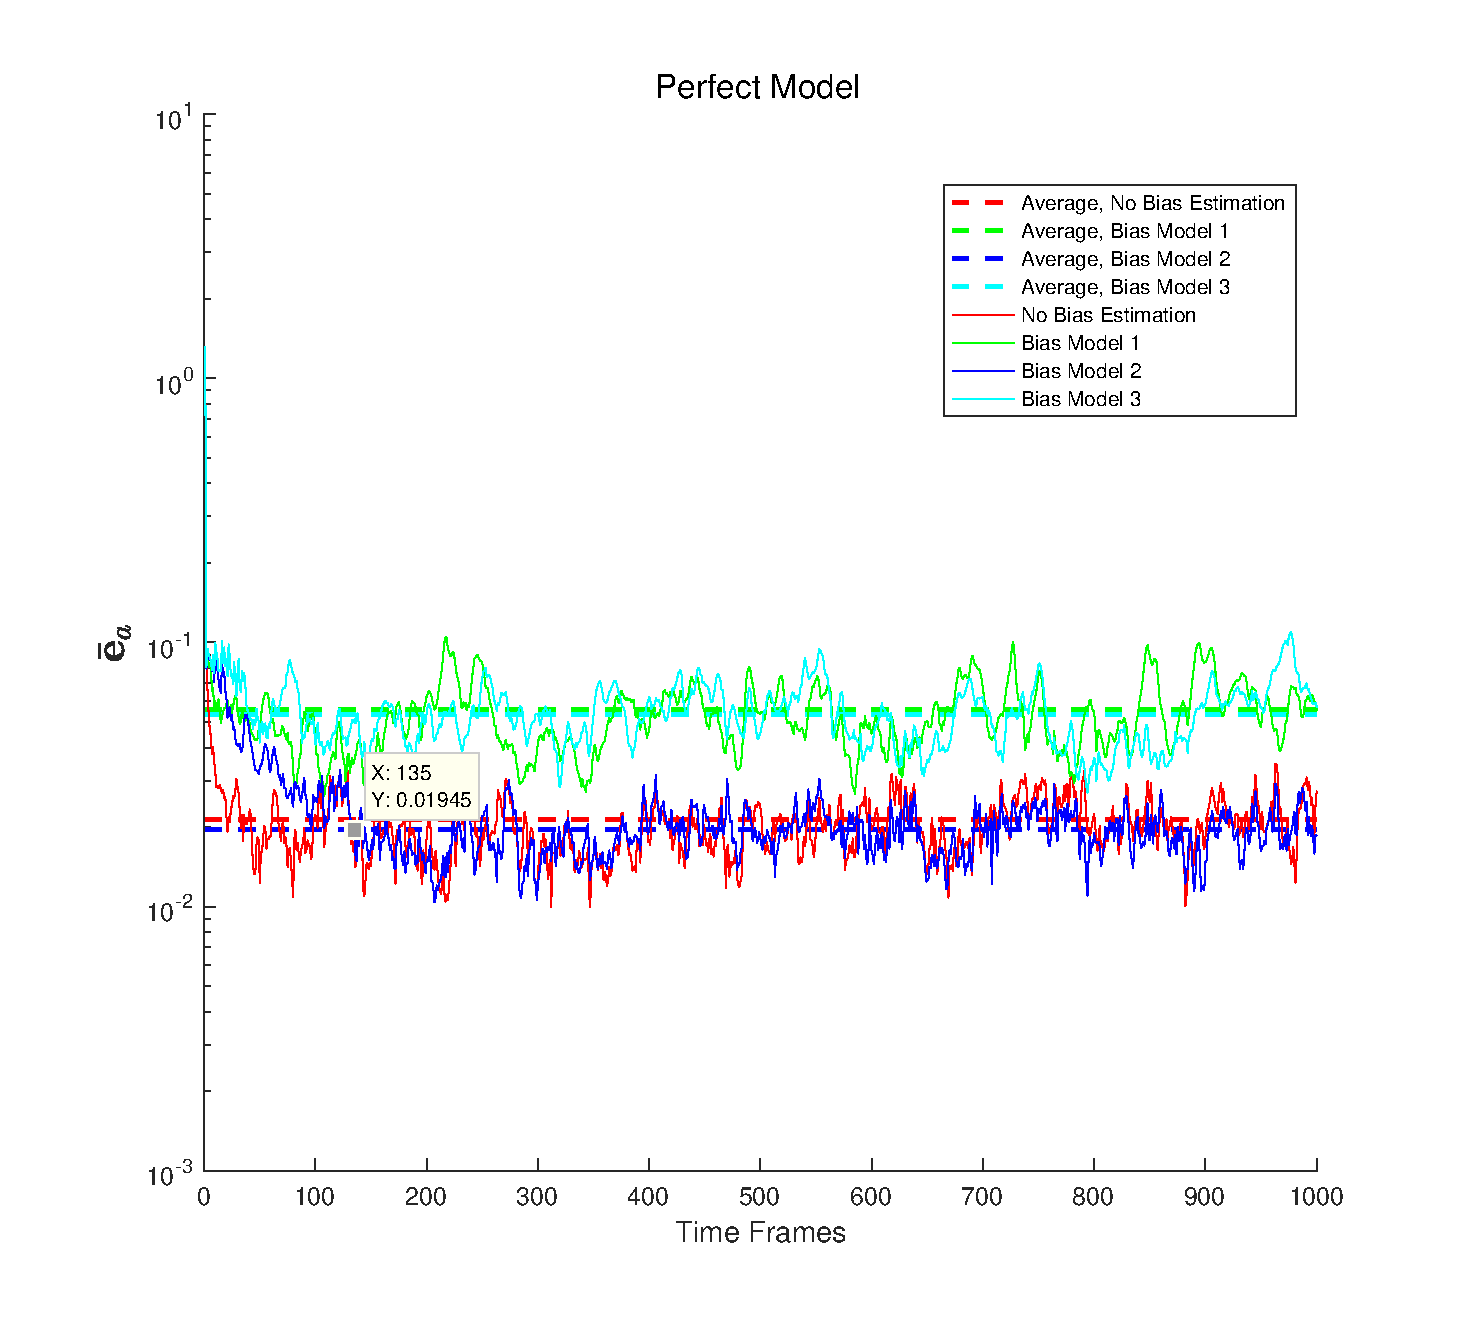
\includegraphics[scale=0.4]{Figures/ErrVsTimeP1}
\end{figure}
\end{frame}

\begin{frame}
\frametitle{Perfect Situation: Performance and Inflation}
\begin{figure} 
\centering
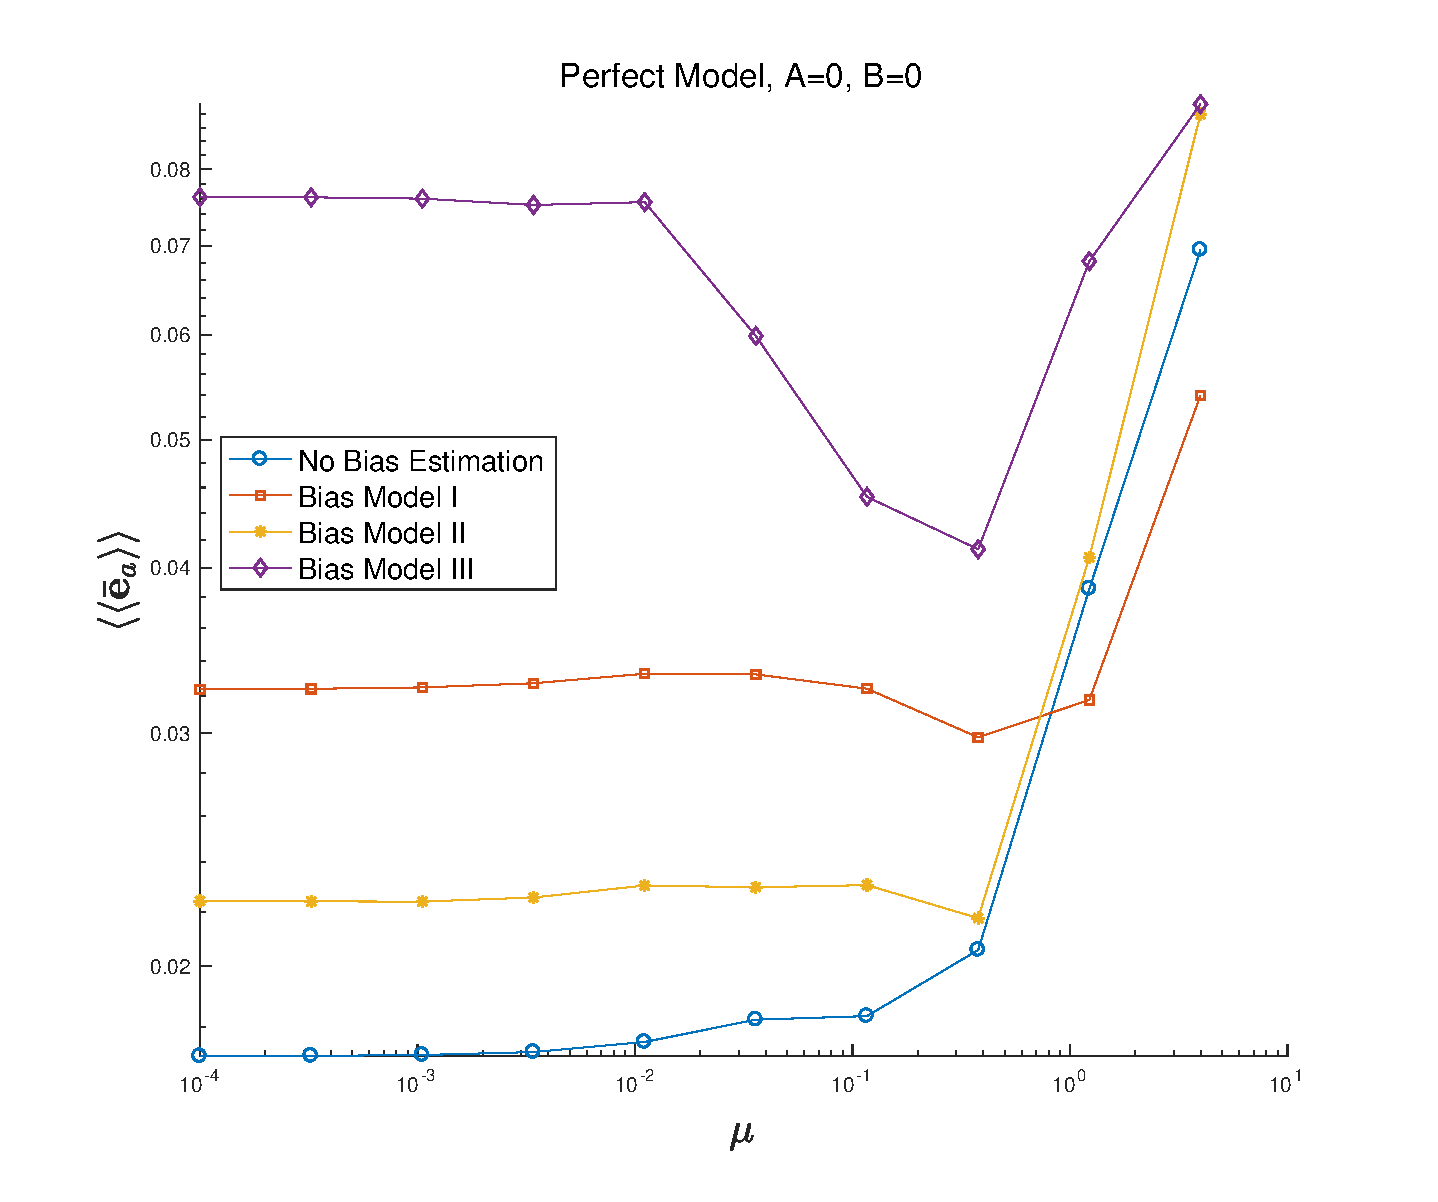
\includegraphics[scale=0.4]{Figures/AErrVsMuP1}
\end{figure}
\end{frame}

\begin{frame}
\frametitle{Perfect Situation: Bias Estimation}
\begin{figure} 
\centering
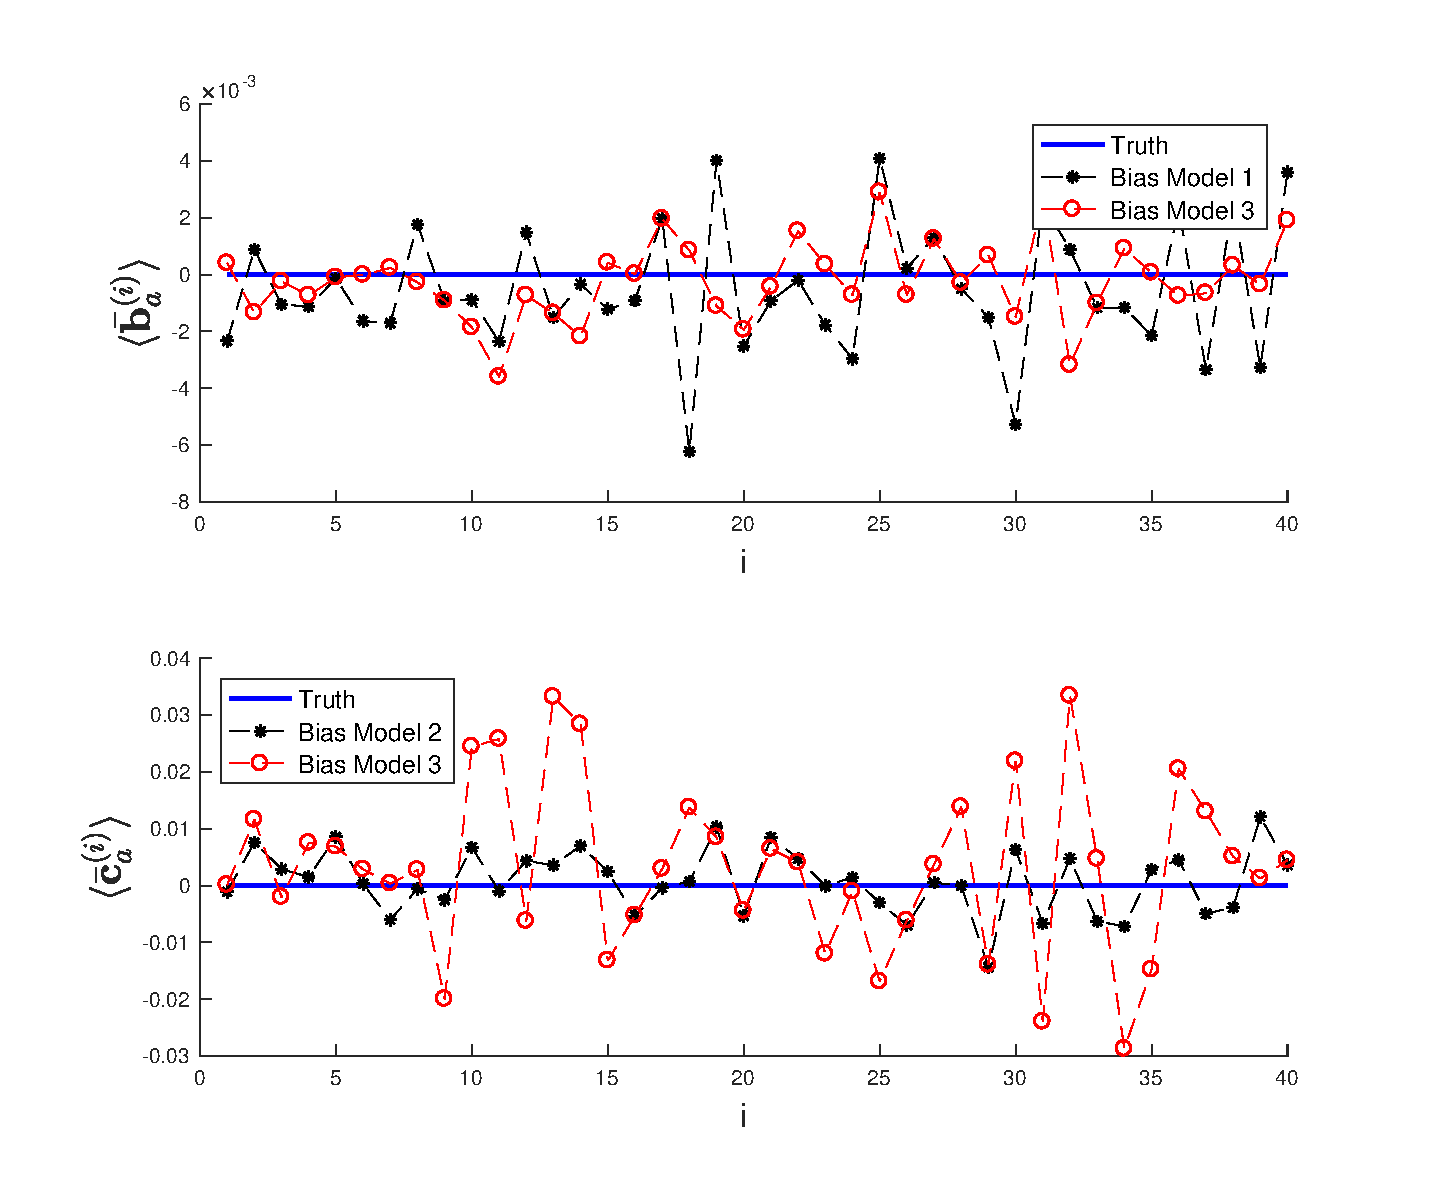
\includegraphics[scale=0.4]{Figures/BiasEstP1}
\end{figure}
\end{frame}

\begin{frame}
\frametitle{Type I Model Error: Settling Time for Error}
\begin{figure} 
\centering
\includegraphics[scale=0.4]{Figures/ErrVsTimeM1_1}
\end{figure}
\end{frame}

\begin{frame}
\frametitle{Type I Model Error: Performance and Inflation}
\begin{figure} 
\centering
\includegraphics[scale=0.4]{Figures/AErrVsMuM1_1}
\end{figure}
\end{frame}

\begin{frame}
\frametitle{Type I Model Error: Bias Estimation}
\begin{figure} 
\centering
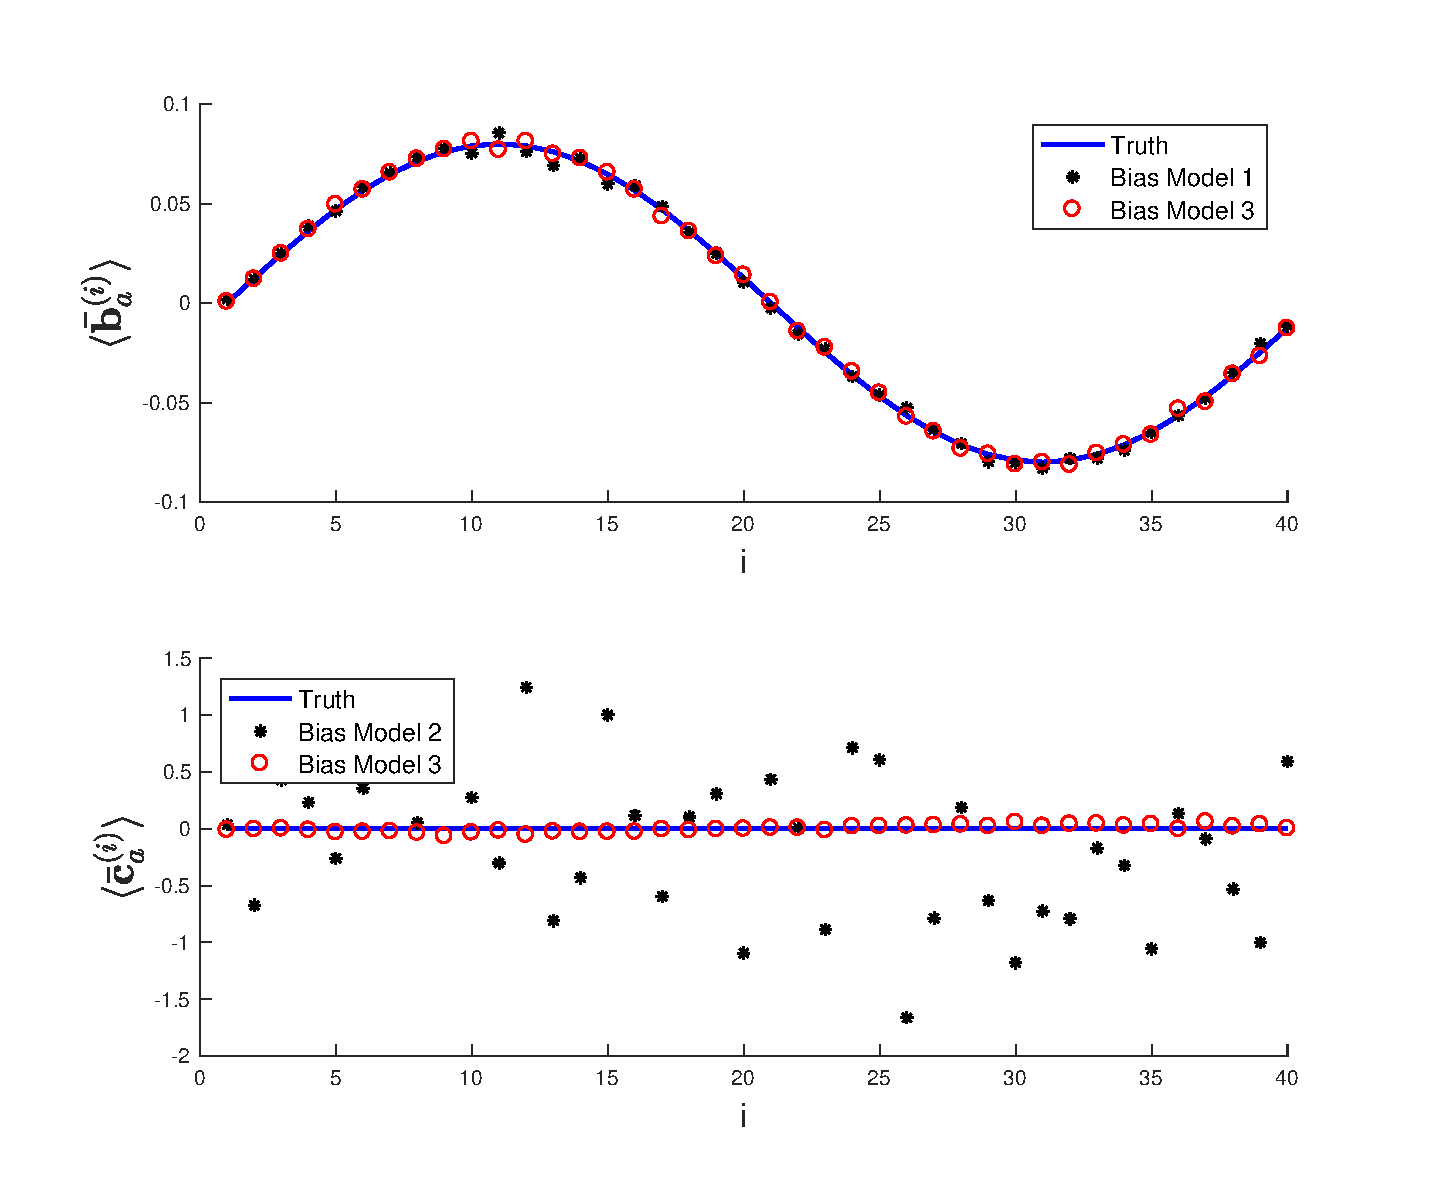
\includegraphics[scale=0.4]{Figures/BiasEstM1}
\end{figure}
\end{frame}

\begin{frame}
\frametitle{Type II Model Error: Settling Time for Error}
\begin{figure} 
\centering
\includegraphics[scale=0.4]{Figures/ErrVsTimeM2_1}
\end{figure}
\end{frame}

\begin{frame}
\frametitle{Type II Model Error: Performance and Inflation}
\begin{figure} 
\centering
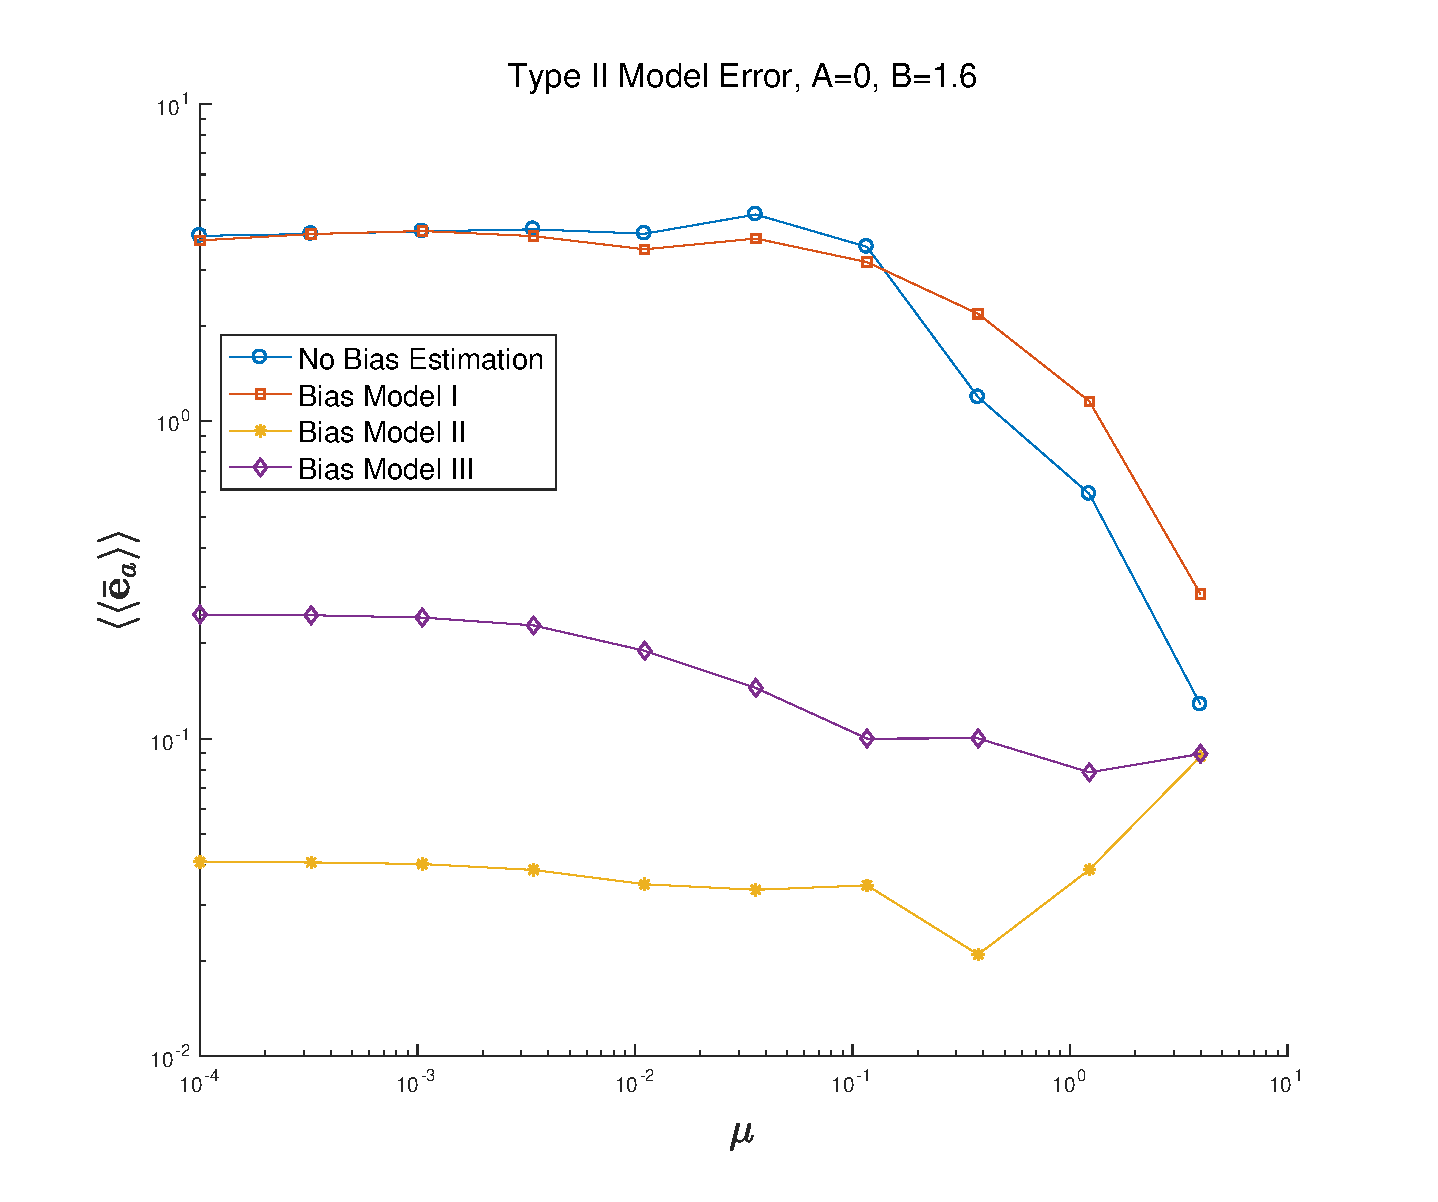
\includegraphics[scale=0.4]{Figures/AErrVsMuM2_1}
\end{figure}
\end{frame}

\begin{frame}
\frametitle{Type II Model Error: Bias Estimation}
\begin{figure} 
\centering
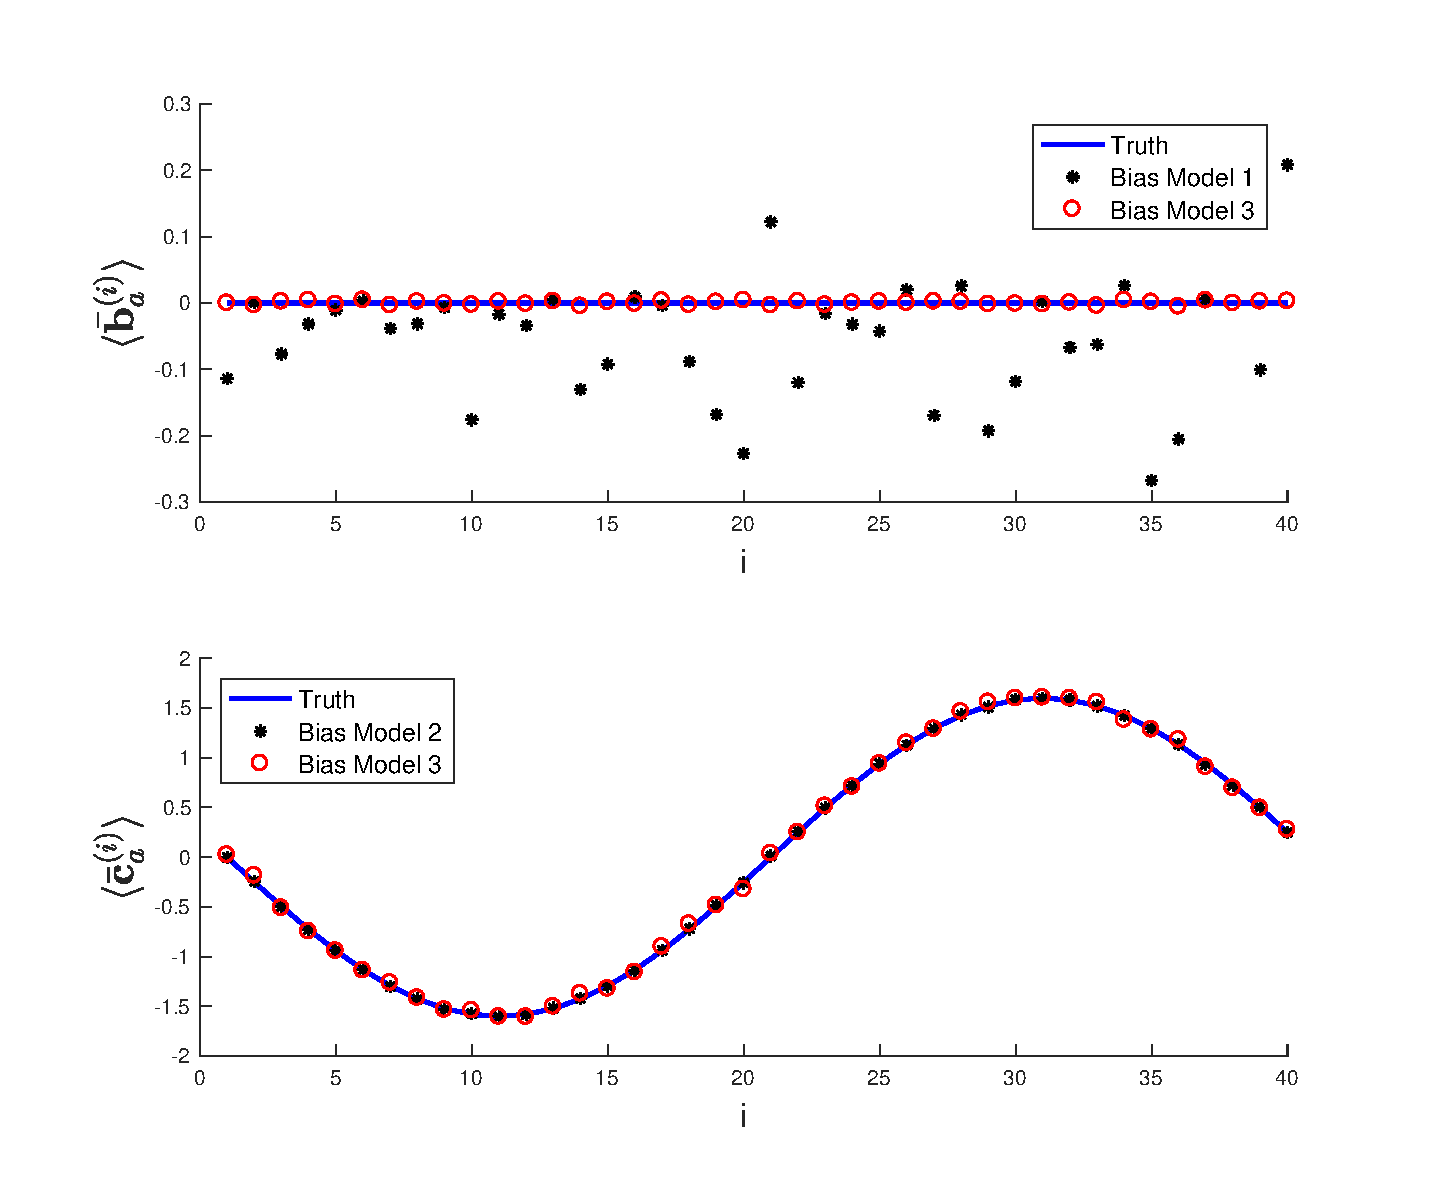
\includegraphics[scale=0.4]{Figures/BiasEstM2}
\end{figure}
\end{frame}

\begin{frame}
\frametitle{Type III Model Error: Settling Time for Error}
\begin{figure} 
\centering
\includegraphics[scale=0.4]{Figures/ErrVsTimeM3_1}
\end{figure}
\end{frame}

\begin{frame}
\frametitle{Type III Model Error: Performance and Inflation}
\begin{figure} 
\centering
\includegraphics[scale=0.4]{Figures/AErrVsMuM3_1}
\end{figure}
\end{frame}

\begin{frame}
\frametitle{Type III Model Error: Bias Estimation}
\begin{figure} 
\centering
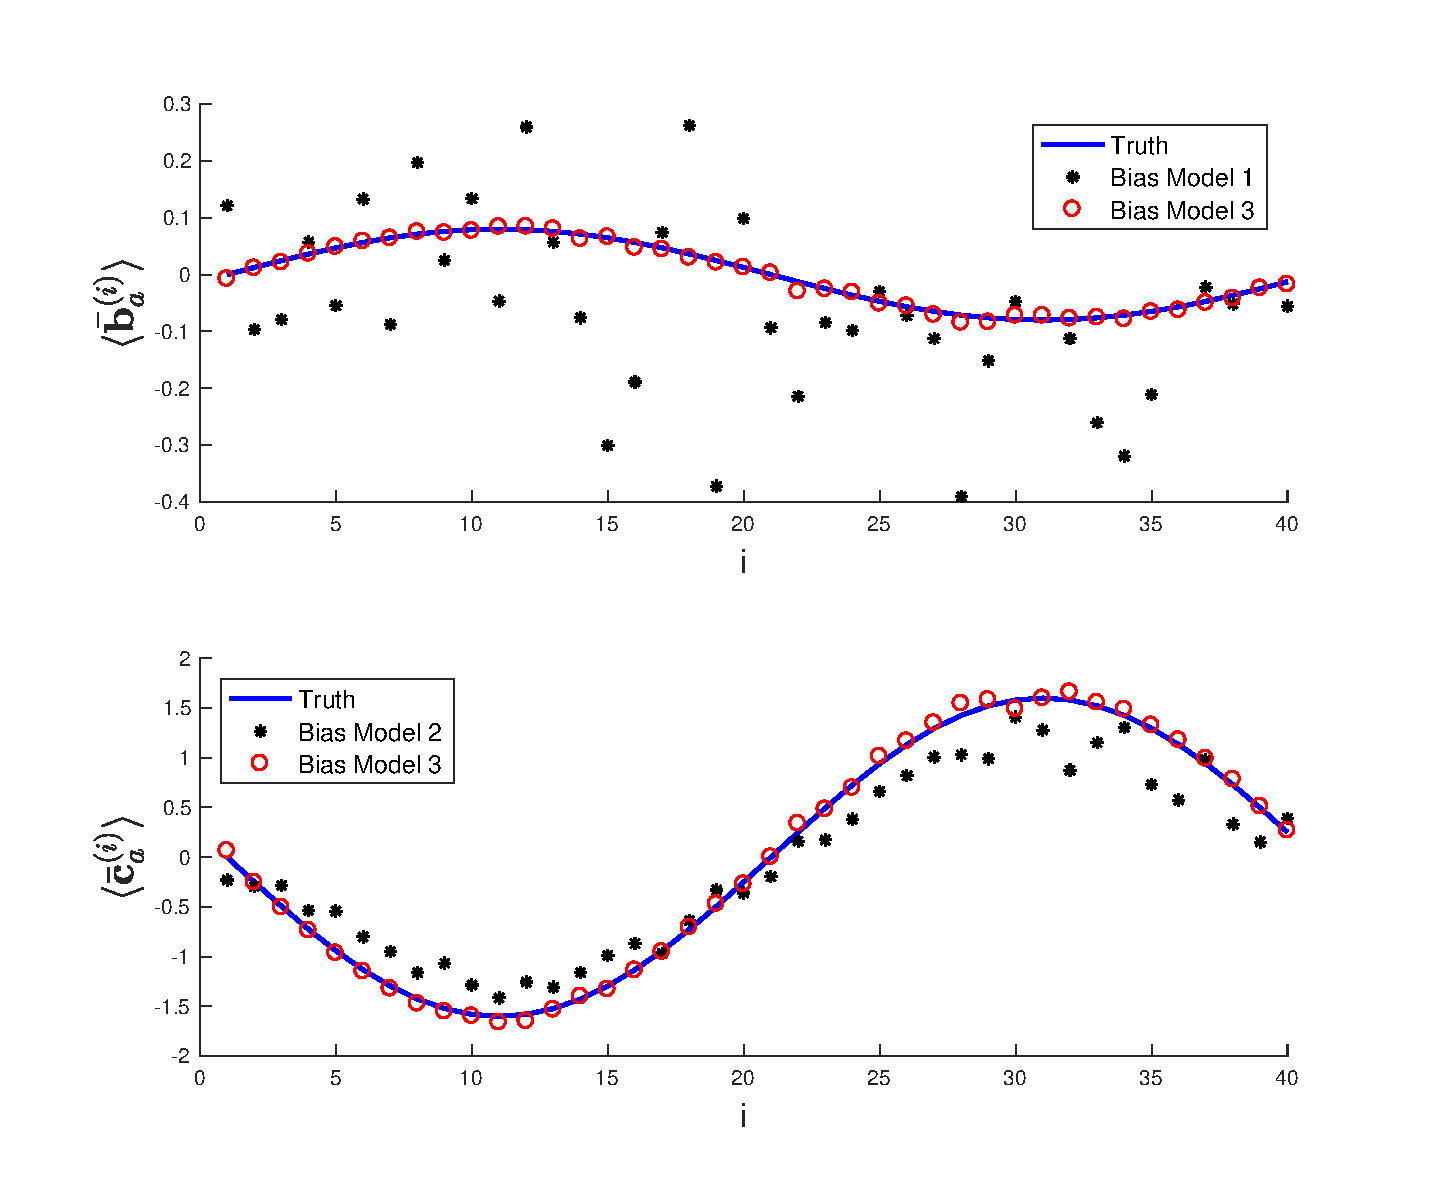
\includegraphics[scale=0.4]{Figures/BiasEstM3}
\end{figure}
\end{frame}



\end{document}